\documentclass[12pt,a4paper]{article}
\usepackage{geometry}
\geometry{left=2.5cm,right=2.5cm,top=2.5cm,bottom=2.5cm}
\usepackage{times}
\usepackage{amsmath,amssymb}
\usepackage{graphicx}
% Graphics path for all figures
\graphicspath{{figure/}}
\usepackage{booktabs}
\usepackage{hyperref}
\usepackage{enumitem}
\usepackage{array}
\usepackage{multirow}
\usepackage{float}
\usepackage{tikz}
\usetikzlibrary{arrows.meta,positioning,calc,shapes.geometric}
\usepackage{pgfplots} \pgfplotsset{compat=1.18}
\hypersetup{
  colorlinks=true,
  linkcolor=blue,
  urlcolor=blue,
  citecolor=blue
}

\title{\textbf{A Scalable Hierarchical Wireless Power Transfer System Based on Reconfigurable Intelligent Surfaces for Complex-Environment Wireless Sensor Networks}}
\author{WSN S3 Project Team}
\date{\today}

\begin{document}
\maketitle

\begin{abstract}
Large-scale Wireless Sensor Networks (WSNs) deployed in mountains, forests, industrial sites, and other complex environments face a fundamental challenge: long-term sustainable energy supply. Traditional approaches such as batteries and solar harvesting are unreliable in shaded, occluded, or non-line-of-sight (NLOS) scenarios. Meanwhile, long-range Radio Frequency Wireless Power Transfer (RF WPT) suffers from severe path loss in obstructed terrains, and Magnetic Resonant Coupling (MRC) WPT is highly sensitive to coil misalignment, limiting its robustness in outdoor applications.

This project proposes a scalable and extensible \textbf{hierarchical hybrid WPT architecture} supported by \textbf{Reconfigurable Intelligent Surfaces (RIS)}. At the global layer, multiple RIS panels form controllable multi-hop reflective power pathways enabling long-range RF energy routing across mountains or obstacles. At the local (cluster) layer, programmable metasurfaces act as \textbf{near-field energy lenses}, enhancing magnetic coupling efficiency and misalignment tolerance for MRC WPT. At the network layer, a unified \textbf{RF--RIS--MRC–WSN energy flow model} coordinates end-to-end energy delivery.

The proposed system is not only energy efficient but also inherently \textbf{scalable} (supporting large-scale WSN expansion) and \textbf{extensible} (compatible with UAV-mounted RIS, mobile robots, 6G IoE networks, and future intelligent energy infrastructure). The project integrates theoretical modeling, electromagnetic simulation, hardware prototyping, and systematic validation to deliver an engineering-ready wireless energy ecosystem.
\end{abstract}

\tableofcontents

\section{Background and Significance}

\subsection{Background}

WSNs are widely deployed for environmental monitoring, agriculture, forest fire prevention, border surveillance, and industrial equipment management. However, in real-world terrain—mountains, forests, canyons—WSN nodes face severe limitations:

\begin{itemize}
  \item \textbf{Unpredictable energy availability}: solar energy fluctuates heavily due to terrain occlusion.
  \item \textbf{No line-of-sight RF conditions}: mountains and obstacles drastically attenuate WPT signals.
  \item \textbf{Maintenance costs}: manually replacing batteries is infeasible for large-scale deployments.
  \item \textbf{Harsh spatial constraints}: MRC WPT cannot maintain efficiency under coil misalignment, tilting, or movement.
\end{itemize}

Recent progress in RIS offers a new opportunity: using programmable metasurfaces to engineer electromagnetic propagation for both long-range and near-field energy transfer.

% Figure: real deployment context (terrain + sun/photoperiod constraints)
\begin{figure}[H]
  \centering
  \includegraphics[width=0.8\textwidth]{实际部署场景.png}
  \caption{Real-world deployment context: mountainous terrain and seasonal sun-path constraints relevant to WSN energy availability.}
  \label{fig:terrain-sun}
\end{figure}

\subsection{Significance}

This project integrates RF WPT, MRC WPT, and RIS into a \textbf{multi-layer, multi-scale hybrid WPT ecosystem}, addressing both long-range reachability and local high-efficiency power delivery.

Significance includes:

\begin{enumerate}
  \item \textbf{Solving NLOS long-range power delivery} via RIS-based controllable RF energy routing.
  \item \textbf{Enhancing near-field coupling efficiency} using RIS as a magnetic energy lens.
  \item \textbf{Establishing a unified cross-layer energy flow framework} for RF--RIS--MRC--WSN.
  \item \textbf{Supporting scalable WSN deployments}: RIS-assisted power networks can expand seamlessly with network size.
  \item \textbf{Providing extensibility to future intelligent energy systems}: RIS-enabled energy routing can interface with UAVs, mobile robots, and 6G IoE smart environments.
\end{enumerate}

\section{Related Work and Limitations}

\subsection{RIS-assisted RF Wireless Power Transfer}

Existing studies show that RIS can improve RF WPT performance by redirecting and focusing incident waves. However:

\begin{itemize}
  \item Most work focuses on \textbf{single RIS panels} in indoor scenarios.
  \item Very limited research addresses \textbf{multi-RIS cooperative power routing}.
  \item No existing work handles \textbf{mountainous terrains or multi-obstacle outdoor environments}.
\end{itemize}

% Figure: self-powered RIS concept as forward-looking enhancement
\begin{figure}[H]
  \centering
  \includegraphics[width=0.92\textwidth]{自供电式RIS.png}
  \caption{Self-powered reconfigurable intelligent metasurface concept, enabling autonomous operation for outdoor deployments.}
  \label{fig:self-powered-ris}
\end{figure}

\subsection{Metasurface-enhanced Magnetic Resonant Coupling}

Metasurfaces have been tested to improve magnetic coupling efficiency, but:

\begin{itemize}
  \item Studies mainly use fixed, non-programmable metasurfaces.
  \item Theoretical understanding of \textbf{near-field focusing and misalignment compensation} is incomplete.
  \item Integration with real WSN deployments is missing.
\end{itemize}

\subsection{Energy Management in WSNs}

Traditional energy scheduling approaches (harvesting-oriented, SWIPT, duty-cycling) are not sufficient because:

\begin{itemize}
  \item They assume limited or uncontrollable energy inflow.
  \item They do not consider \textbf{joint RF–MRC energy flows}.
  \item None incorporate RIS as an active energy-routing infrastructure.
\end{itemize}

\subsection{Gaps Addressed by This Project}

The project targets the following gaps:

\begin{enumerate}
  \item Multi-RIS cooperative \textbf{energy routing} across non-line-of-sight terrains.
  \item RIS-enabled \textbf{magnetic energy lensing} for robust MRC power transfer.
  \item A unified \textbf{cross-layer energy flow model}.
  \item A \textbf{scalable and extensible WPT architecture} for real-world large-scale WSNs.
\end{enumerate}

\section{Key Scientific Problem}

The core scientific challenge of this project can be summarized as:

\begin{quote}
\textbf{How to design, model, and optimize a scalable hierarchical RF--RIS--MRC wireless power transfer system that can reliably deliver energy across complex non-line-of-sight environments and efficiently power large-scale WSN deployments, while coordinating long-range RF energy routing and near-field magnetic resonant charging in a unified framework?}
\end{quote}

This overarching problem naturally decomposes into the following tightly coupled subproblems.

\subsection*{Subproblem 1: Multi-RIS Cooperative Energy Routing in NLOS Environments}

How can we construct and optimize multi-hop, RIS-assisted RF energy paths in complex terrains where direct line-of-sight links do not exist?

\begin{itemize}
  \item How to model multi-RIS cascaded reflective channels over real terrain (e.g., mountains, obstacles) and incorporate terrain elevation and shadowing into energy routing?
  \item How to jointly design energy routing paths and RIS phase configurations to maximize received power, minimize path loss, or balance energy among multiple clusters?
  \item How to maintain robustness against environmental changes (e.g., foliage, partial blockage) and support scalable extension to additional RIS panels and WSN clusters?
\end{itemize}

% Figure: RIS-assisted RF power routing in mountainous terrain
\begin{figure}[H]
  \centering
  \includegraphics[width=\textwidth]{场景示意图.png}
  \caption{RIS-assisted RF power routing in mountainous terrain: incident and reflected paths across adret and nightside slopes.}
  \label{fig:ris-routing}
\end{figure}

\subsection*{Subproblem 2: RIS-enhanced MRC for Near-field Energy Focusing and Robustness}

How can programmable metasurfaces be used as near-field energy lenses to enhance magnetic resonant coupling efficiency and misalignment tolerance within each cluster?

\begin{itemize}
  \item What are the underlying mechanisms by which RIS structures reshape the near-field magnetic distribution and improve the coupling coefficient, quality factor, and end-to-end efficiency?
  \item How do RIS structural parameters (unit cell geometry, periodicity, material properties) affect the trade-off between focusing strength, efficiency, and robustness to coil displacement and rotation?
  \item How can we design adaptive RIS control patterns that compensate for spatial drift or position uncertainty of sensor nodes in realistic deployments?
\end{itemize}

\section{Technical Route and Methodology}

\subsection{Overall Technical Route}

The project follows a five-stage methodology:

\begin{enumerate}
  \item Multi-RIS RF energy routing modeling.
  \item RIS-enhanced MRC near-field focusing and robustness study.
  \item Unified hierarchical energy-flow model construction.
  \item Hardware prototyping and system-level experiments.
  \item Scalability and extensibility evaluation.
\end{enumerate}

\subsection{Multi-RIS RF Energy Routing}

\begin{itemize}
  \item Construct geometric and electromagnetic models for cascaded RIS-assisted RF WPT.
  \item Integrate terrain elevation maps (DEM) into routing graphs.
  \item Optimize routing via dynamic programming, graph search, or ADMM-based joint phase-path optimization.
\end{itemize}

\subsection{RIS-enhanced MRC Energy Lens}

\begin{itemize}
  \item Use HFSS/CST to simulate magnetic field shaping under programmable RIS.
  \item Analyze coupling coefficient $k$, Q-factor, and efficiency $\eta$ under misalignment.
  \item Develop adaptive RIS control patterns for moving or drifting nodes.
\end{itemize}

% Figure: Near-field magnetic energy lensing for MRC enhancement
\begin{figure}[H]
  \centering
  \includegraphics[width=\textwidth]{RIS能量透镜.png}
  \caption{Metasurface energy lens for near-field magnetic coupling enhancement in MRC WPT.}
  \label{fig:energy-lens}
\end{figure}

\subsection{Cross-layer Energy Flow Coordination}

\begin{itemize}
  \item Build a unified RF--RIS--MRC--WSN energy-flow graph.
  \item Define energy constraints at each layer.
  \item Design a joint optimization algorithm for global power allocation and local power redistribution.
\end{itemize}

% Figure: Polarization multiplexing for power vs. information separation
\begin{figure}[H]
  \centering
  \includegraphics[width=0.9\textwidth]{极化分集技术.png}
  \caption{Polarization multiplexing concept: orthogonal polarizations carry power (E$_x$) and information (E$_y$) simultaneously.}
  \label{fig:polarization}
\end{figure}

% Figure: Dual-band SWIPT architecture for sensors
\begin{figure}[H]
  \centering
  \includegraphics[width=0.9\textwidth]{双频SWIPT系统.png}
  \caption{Dual-band SWIPT system architecture for IoT/biomedical sensors within the hierarchical WPT network.}
  \label{fig:swipt}
\end{figure}

\section{Experimental Design and Validation Metrics}

\subsection{Experiment 1: Multi-RIS RF Power Routing}

Metrics:

\begin{itemize}
  \item Received power improvement (dB).
  \item Routing stability and reconfigurability.
  \item Multi-RIS cooperative gain vs. number of panels.
\end{itemize}

\subsection{Experiment 2: RIS-enhanced MRC Power Transfer}

Metrics:

\begin{itemize}
  \item Coupling coefficient improvement.
  \item Misalignment tolerance (cm, degrees).
  \item Efficiency enhancement in dynamic scenarios.
\end{itemize}

\subsection{Experiment 3: Hierarchical WPT + WSN Performance}

Metrics:

\begin{itemize}
  \item Node online ratio.
  \item Network lifetime extension.
  \item Energy-balancing performance across clusters.
\end{itemize}

\subsection{Experiment 4: System Scalability and Extensibility}

Evaluate:

\begin{itemize}
  \item Scalability with number of nodes and RIS panels.
  \item Compatibility with mobile RIS (e.g., UAV-mounted).
  \item Integration with 6G IoE or digital-twin-based energy orchestration.
\end{itemize}

% 需要的宏包:
% \usepackage{tikz}
% \usetikzlibrary{arrows.meta,positioning,calc}

\begin{figure}[htbp]
  \centering
  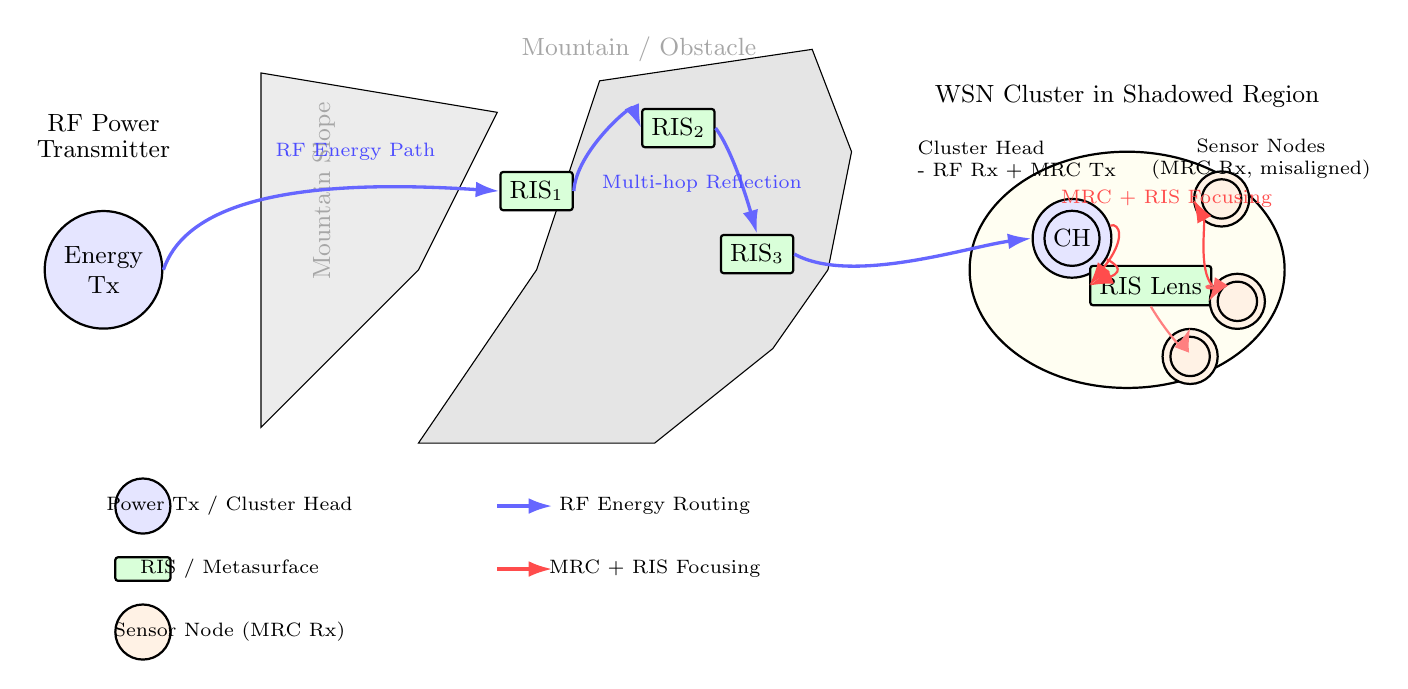
\begin{tikzpicture}[
      scale=1.0,
      every node/.style={font=\small},
      tx/.style={circle,draw,thick,fill=blue!10},
      rx/.style={circle,draw,thick,fill=orange!10},
      ris/.style={rectangle,draw,thick,fill=green!15,rounded corners=1pt},
      cluster/.style={ellipse,draw,thick,fill=yellow!5},
      >={Latex[length=3mm,width=2mm]}
  ]
  
  % ===================== 左侧:Energy Transmitter =====================
  % Use shortstack to allow line breaks inside TikZ nodes without LR-mode issues
  \node[tx, minimum size=1.1cm] (txnode) at (-6,0) {\shortstack{Energy\\Tx}};
  
  \node[align=center] at (-6,1.7) {\shortstack{RF Power\\Transmitter}};
  
  % 画左侧“山坡”
  \draw[fill=gray!15] (-4,-2) -- (-2,0) -- (-1,2) -- (-4,2.5) -- cycle;
  \node[rotate=90,gray!70] at (-3.2,1.0) {Mountain Slope};
  
  % ===================== 中间:山体 + 多块 RIS =====================
  
  % 山体主体
  \draw[fill=gray!20] (-2.0,-2.2) -- (-0.5,0) -- (0,1.5) -- (0.3,2.4) -- (3.0,2.8)
                      -- (3.5,1.5) -- (3.2,0) -- (2.5,-1.0) -- (1.0,-2.2) -- cycle;
  \node[gray!70] at (0.8,2.8) {Mountain / Obstacle};
  
  % 三块 RIS
  \node[ris,minimum width=0.9cm,minimum height=0.4cm] (ris1) at (-0.5,1.0) {RIS$_1$};
  \node[ris,minimum width=0.9cm,minimum height=0.4cm] (ris2) at (1.3,1.8) {RIS$_2$};
  \node[ris,minimum width=0.9cm,minimum height=0.4cm] (ris3) at (2.3,0.2) {RIS$_3$};
  
  % ===================== 右侧:Cluster 区域 =====================
  
  % 簇区域
  \node[cluster,minimum width=4cm,minimum height=3.0cm] (cluster) at (7,0) {};
  
  \node[align=center] at (7,2.2) {WSN Cluster in Shadowed Region};
  
  % 簇头 CH
  \node[tx,minimum size=1.0cm] (ch) at (6.3,0.4) {CH};
  
  \node[align=left,font=\scriptsize] at (5.6,1.4) {Cluster Head\\- RF Rx + MRC Tx};
  
  % 簇内 RIS / Metasurface Lens
  \node[ris,minimum width=1.4cm,minimum height=0.5cm] (inris) at (7.3,-0.2) {RIS Lens};
  
  % 簇内节点(MRC Rx)
  \node[rx,minimum size=0.7cm] (n1) at (8.2,0.9) {};
  \node[rx,minimum size=0.7cm] (n2) at (8.4,-0.4) {};
  \node[rx,minimum size=0.7cm] (n3) at (7.8,-1.1) {};
  
  \node[font=\scriptsize,align=center] at (8.7,1.4)
      {Sensor Nodes\\(MRC Rx, misaligned)};
  
  % 在节点上画小线圈表示 Rx
  \draw[thick] (n1) circle (0.25);
  \draw[thick] (n2) circle (0.25);
  \draw[thick] (n3) circle (0.25);
  
  % 在 CH 上画线圈表示 MRC Tx
  \draw[thick] (6.3,0.4) circle (0.35);
  
  % ===================== 能量路由路径:Tx -> RIS -> CH =====================
  
  % 射线路径:Tx -> RIS1 -> RIS2 -> RIS3 -> CH
  \draw[very thick,blue!60,->]
      (txnode.east) .. controls (-5,0.7) and (-4,1.2) .. (ris1.west);
  
  \draw[very thick,blue!60,->]
      (ris1.east) .. controls (0.0,1.5) and (0.7,2.1) .. (ris2.west);
  
  \draw[very thick,blue!60,->]
      (ris2.east) .. controls (2.0,1.5) and (2.2,0.8) .. (ris3.north);
  
  \draw[very thick,blue!60,->]
      (ris3.east) .. controls (3.5,-0.2) and (5.0,0.3) .. (ch.west);
  
  \node[font=\scriptsize,blue!70] at (-2.8,1.5) {RF Energy Path};
  \node[font=\scriptsize,blue!70] at (1.6,1.1) {Multi-hop Reflection};
  
  % ===================== 簇内 MRC + RIS 透镜示意 =====================
  
  % 簇内磁场线(聚焦)
  \draw[thick,red!70,->] (ch) .. controls (6.8,0.1) and (7.0,0.0) .. (inris.west);
  \draw[thick,red!70,->] (ch) .. controls (6.9,0.6) and (7.0,0.4) .. (inris.west);
  
  \draw[thick,red!70,->] (inris.east) .. controls (7.9,0.0) and (8.0,0.6) .. (n1.west);
  \draw[thick,red!60,->] (inris.east) .. controls (7.9,-0.2) and (8.1,-0.3) .. (n2.west);
  \draw[thick,red!50,->] (inris.south) .. controls (7.5,-0.8) and (7.7,-1.0) .. (n3.north);
  
  \node[font=\scriptsize,red!70] at (7.5,0.9) {MRC + RIS Focusing};
  
  % ===================== 图例(可选) =====================
  \node[tx,minimum size=0.7cm] (legtx) at (-5.5,-3.0) {};
  \node[align=left,font=\scriptsize] at (-4.4,-3.0) {Power Tx / Cluster Head};
  
  \node[ris,minimum width=0.7cm,minimum height=0.3cm] (legris) at (-5.5,-3.8) {};
  \node[align=left,font=\scriptsize] at (-4.4,-3.8) {RIS / Metasurface};
  
  \node[rx,minimum size=0.7cm] (legrx) at (-5.5,-4.6) {};
  \node[align=left,font=\scriptsize] at (-4.4,-4.6) {Sensor Node (MRC Rx)};
  
  \draw[very thick,blue!60,->] (-1.0,-3.0) -- (-0.3,-3.0);
  \node[font=\scriptsize,align=left] at (1.0,-3.0) {RF Energy Routing};
  
  \draw[very thick,red!70,->] (-1.0,-3.8) -- (-0.3,-3.8);
  \node[font=\scriptsize,align=left] at (1.0,-3.8) {MRC + RIS Focusing};
  
  \end{tikzpicture}
  \caption{Overall system architecture: cross-mountain RIS-assisted RF energy routing and intra-cluster RIS-enhanced magnetic resonant wireless power transfer.}
  \label{fig:system_arch}
  \end{figure}
  

  \begin{figure}[htbp]
    \centering
    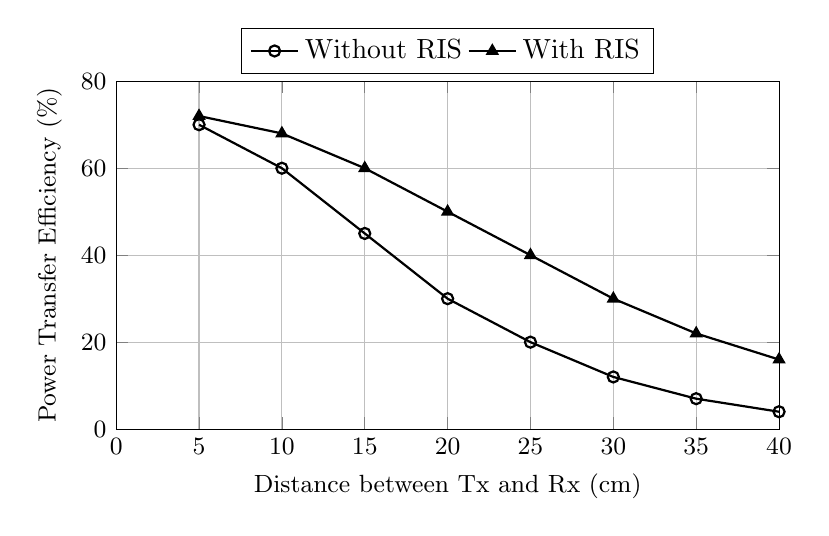
\begin{tikzpicture}
    \begin{axis}[
        width=10cm,
        height=6cm,
        xlabel={Distance between Tx and Rx (cm)},
        ylabel={Power Transfer Efficiency (\%)},
        xmin=0, xmax=40,
        ymin=0, ymax=80,
        grid=both,
        legend style={at={(0.5,1.02)},anchor=south,legend columns=-1},
        legend cell align={left},
        ticklabel style={font=\small},
        label style={font=\small}
    ]
    
    % No RIS curve (示例数据,可换成你自己实验数据)
    \addplot[thick,mark=o] coordinates {
        (5,70)
        (10,60)
        (15,45)
        (20,30)
        (25,20)
        (30,12)
        (35,7)
        (40,4)
    };
    \addlegendentry{Without RIS}
    
    % With RIS curve (示例数据)
    \addplot[thick,mark=triangle*] coordinates {
        (5,72)
        (10,68)
        (15,60)
        (20,50)
        (25,40)
        (30,30)
        (35,22)
        (40,16)
    };
    \addlegendentry{With RIS}
    
    \end{axis}
    \end{tikzpicture}
    \caption{Comparison of power transfer efficiency with and without RIS as distance increases.}
    \label{fig:efficiency_comparison}
    \end{figure}

    

\end{document}
